\section[Отслеживание контакта в случае \textit{mecanum} колеса]{Отслеживание контакта \\ в случае \textit{mecanum} колеса}\label{sect:track_mecanum}

Обозначим угол между осью ролика и плоскостью колеса $\psi$. В конфигурации обычного омни-колеса этот угол равен нулю. Расширим алгоритм отслеживания контакта, описанный выше для случая $\psi = 0$ на конфигурацию \textit{mecanum}, $\psi > 0$. В этом случае, в первую очередь, отметим отличия в геометрической форме роликов. Каждый ролик -- это твердое тело, ограниченное поверхностью вращения некоторой кривой вокруг его оси. В случае $\psi = 0$ эта кривая -- дуга окружности, но при $\psi > 0$, для того, чтобы проекция внешней границы колеса с роликами на его плоскость оставалась окружностью, образующая кривая поверхности ролика становится алгебраической кривой четвертого порядка \cite{Gfrerrer2008}. Для полноты приведем ее параметризацию в координатах $Kxyz$ (см. рис.~\ref{Roller} в разделе~\ref{sect:track_omni}), указанную в \cite{Gfrerrer2008}. В качестве параметра используется угол поворота колеса $\chi \in \left[ -\ddfrac{\pi}{n}, \ddfrac{\pi}{n} \right]$:
\begin{eqnarray*}
    x(\chi) & = & r\ddfrac{\sin^2\psi}{\cos\psi}\mathrm{tg}\chi + l\cos\psi\sin\chi \\
    y(\chi) & = & -\sqrt{\sin^2\psi\mathrm{tg}^2\chi + 1}\left(l\cos\chi - r\right).
\end{eqnarray*}

\begin{figure}[H]
    \centering
    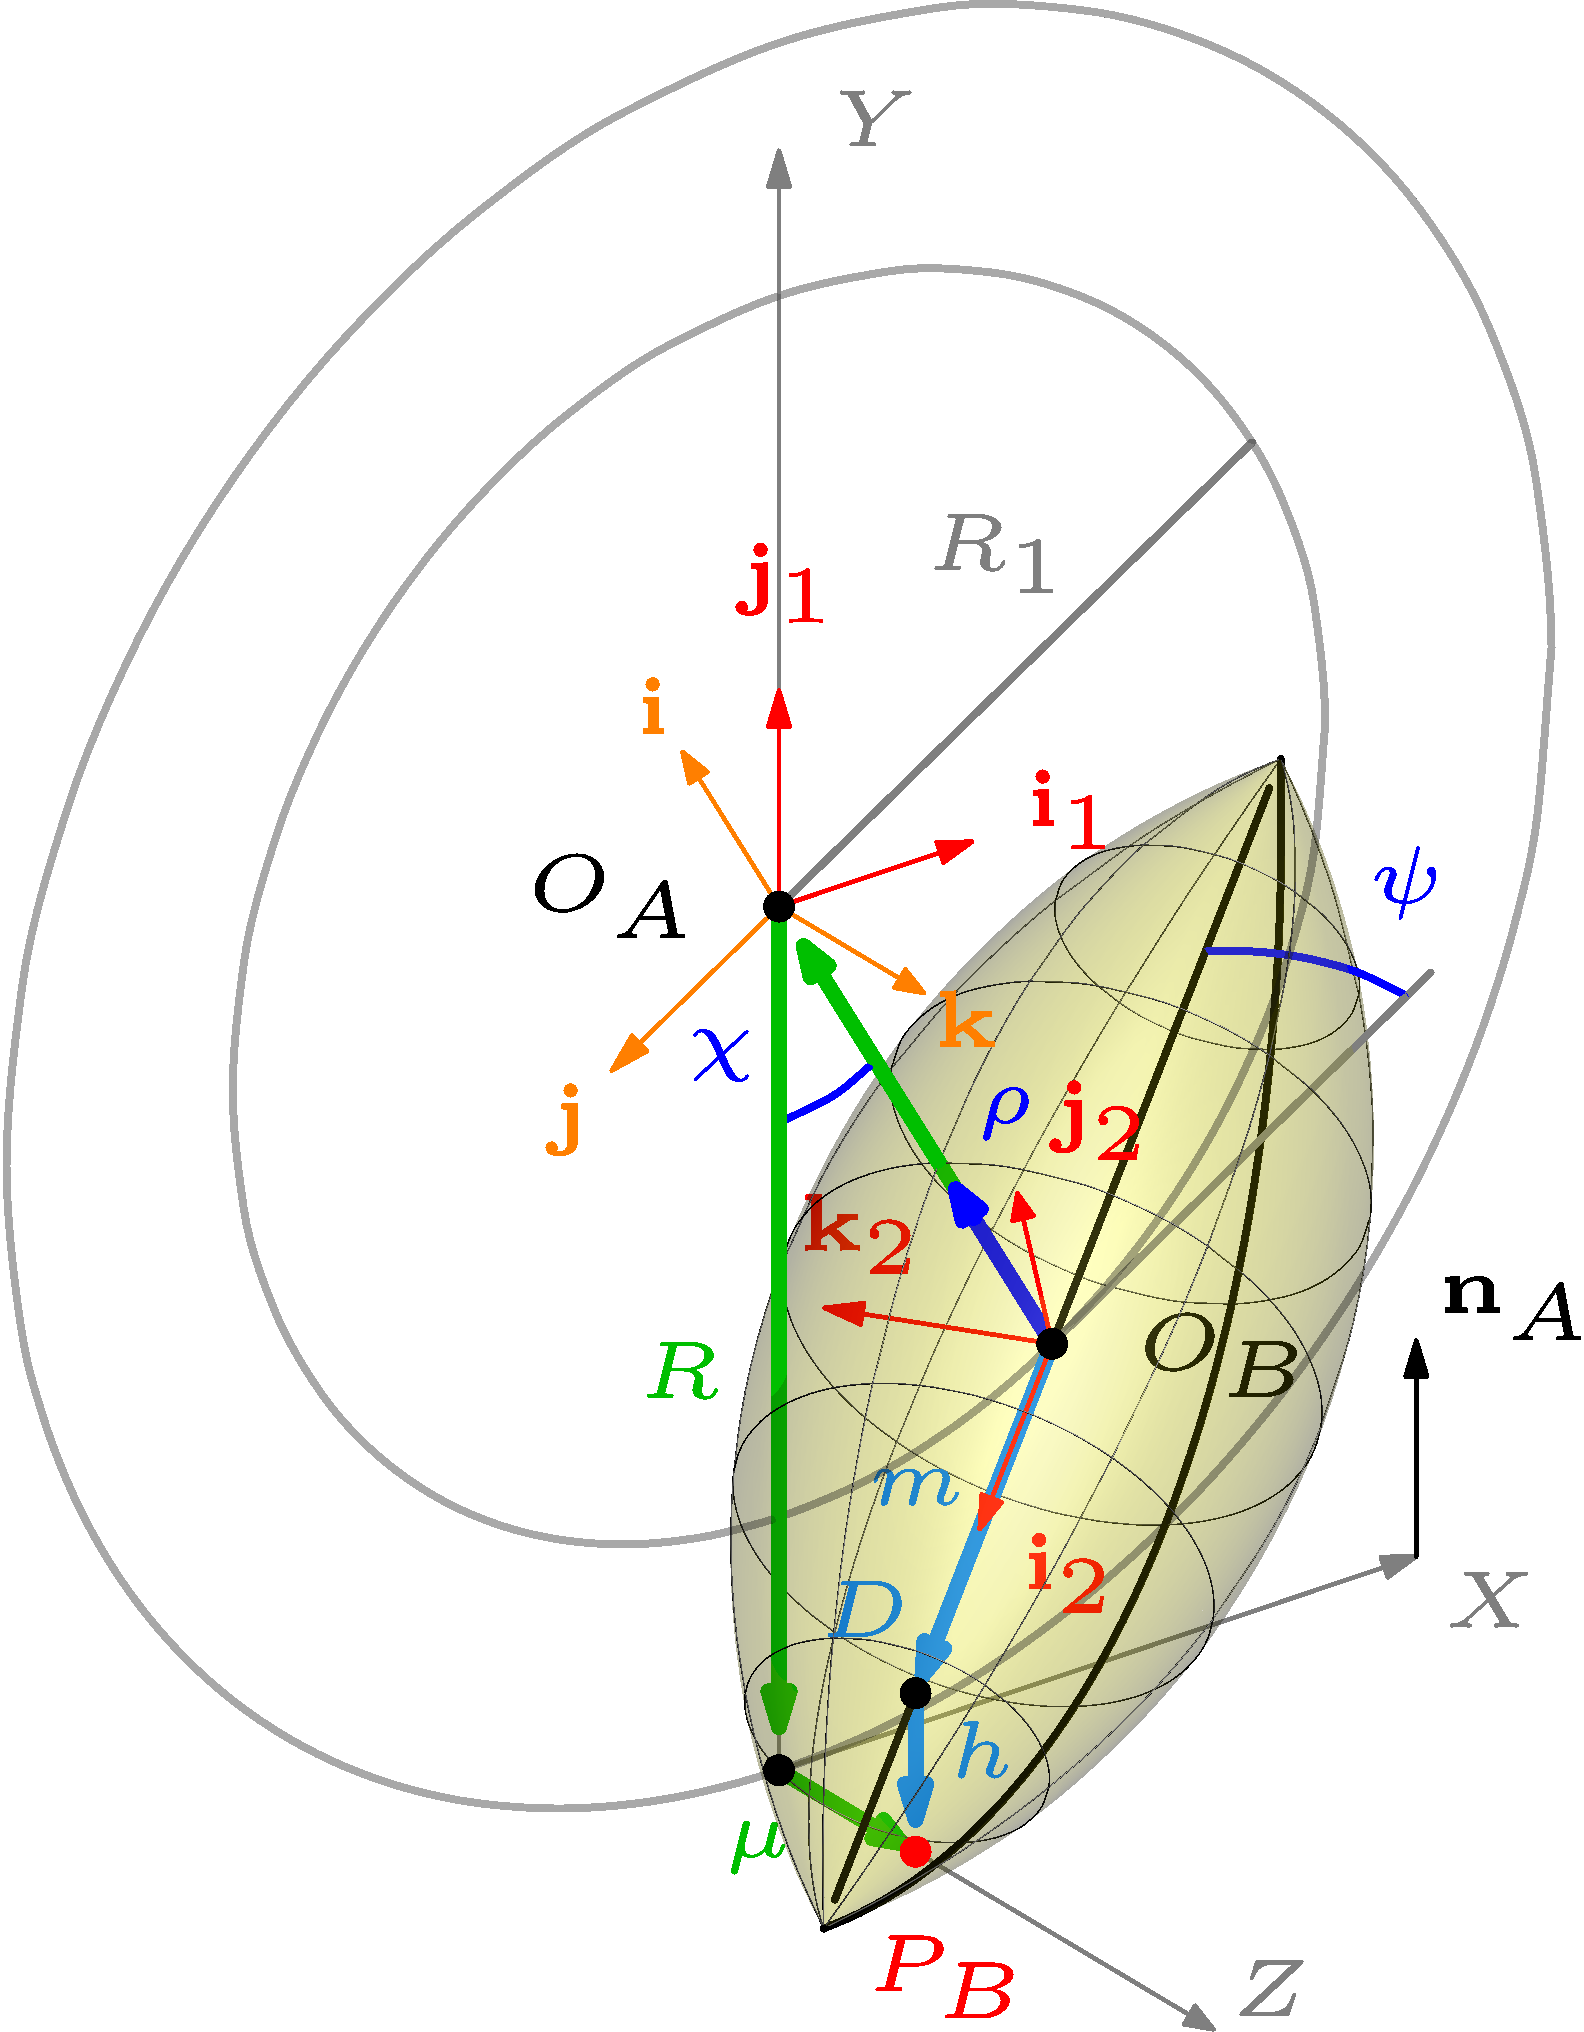
\includegraphics[width=0.75\textwidth]{./content/pic/asy/pic_mecanum.png}
    % \asyinclude[width=0.75\textwidth]{./content/pic/asy/pic_mecanum.asy}
    \caption{Отслеживание контакта для колеса \textit{mecanum}}
    \label{fig:mecanum}
\end{figure}

% \textbf{Неявный алгоритм отслеживания контакта}

% Здесь, как и всюду, будем предполагать, что плоскость колеса вертикальна во все время движения. 
Введем систему отсчета $P{\bf i}{\bf j}{\bf k}$, жестко связанную с колесом (см. рис.~\ref{fig:mecanum}), с началом в его центре $P$. Пусть вектор ${\bf k}$ направлен вдоль оси колеса, ${\bf i}$ и ${\bf j}$ лежат в его плоскости. Введем также две вспомогательные системы отсчета $P{\bf i}_1{\bf j}_1{\bf k}_1$ и $K{\bf i}_2{\bf j}_2{\bf k}_2$, где $K$ -- центр ролика.

Вектор ${\bf i}_2$ направим вдоль оси симметрии ролика, см. рис.~\ref{ContactScheme}. Вектор ${\bf j}_2$ ортогонален ${\bf i}_2$ и лежит в вертикальной плоскости. Третий вектор ${\bf k}_2$ определяется естественным образом как
$$
{\bf k}_2={\bf i}_2\times {\bf j}_2.
$$
% \begin{figure}[hb]
% \centerline{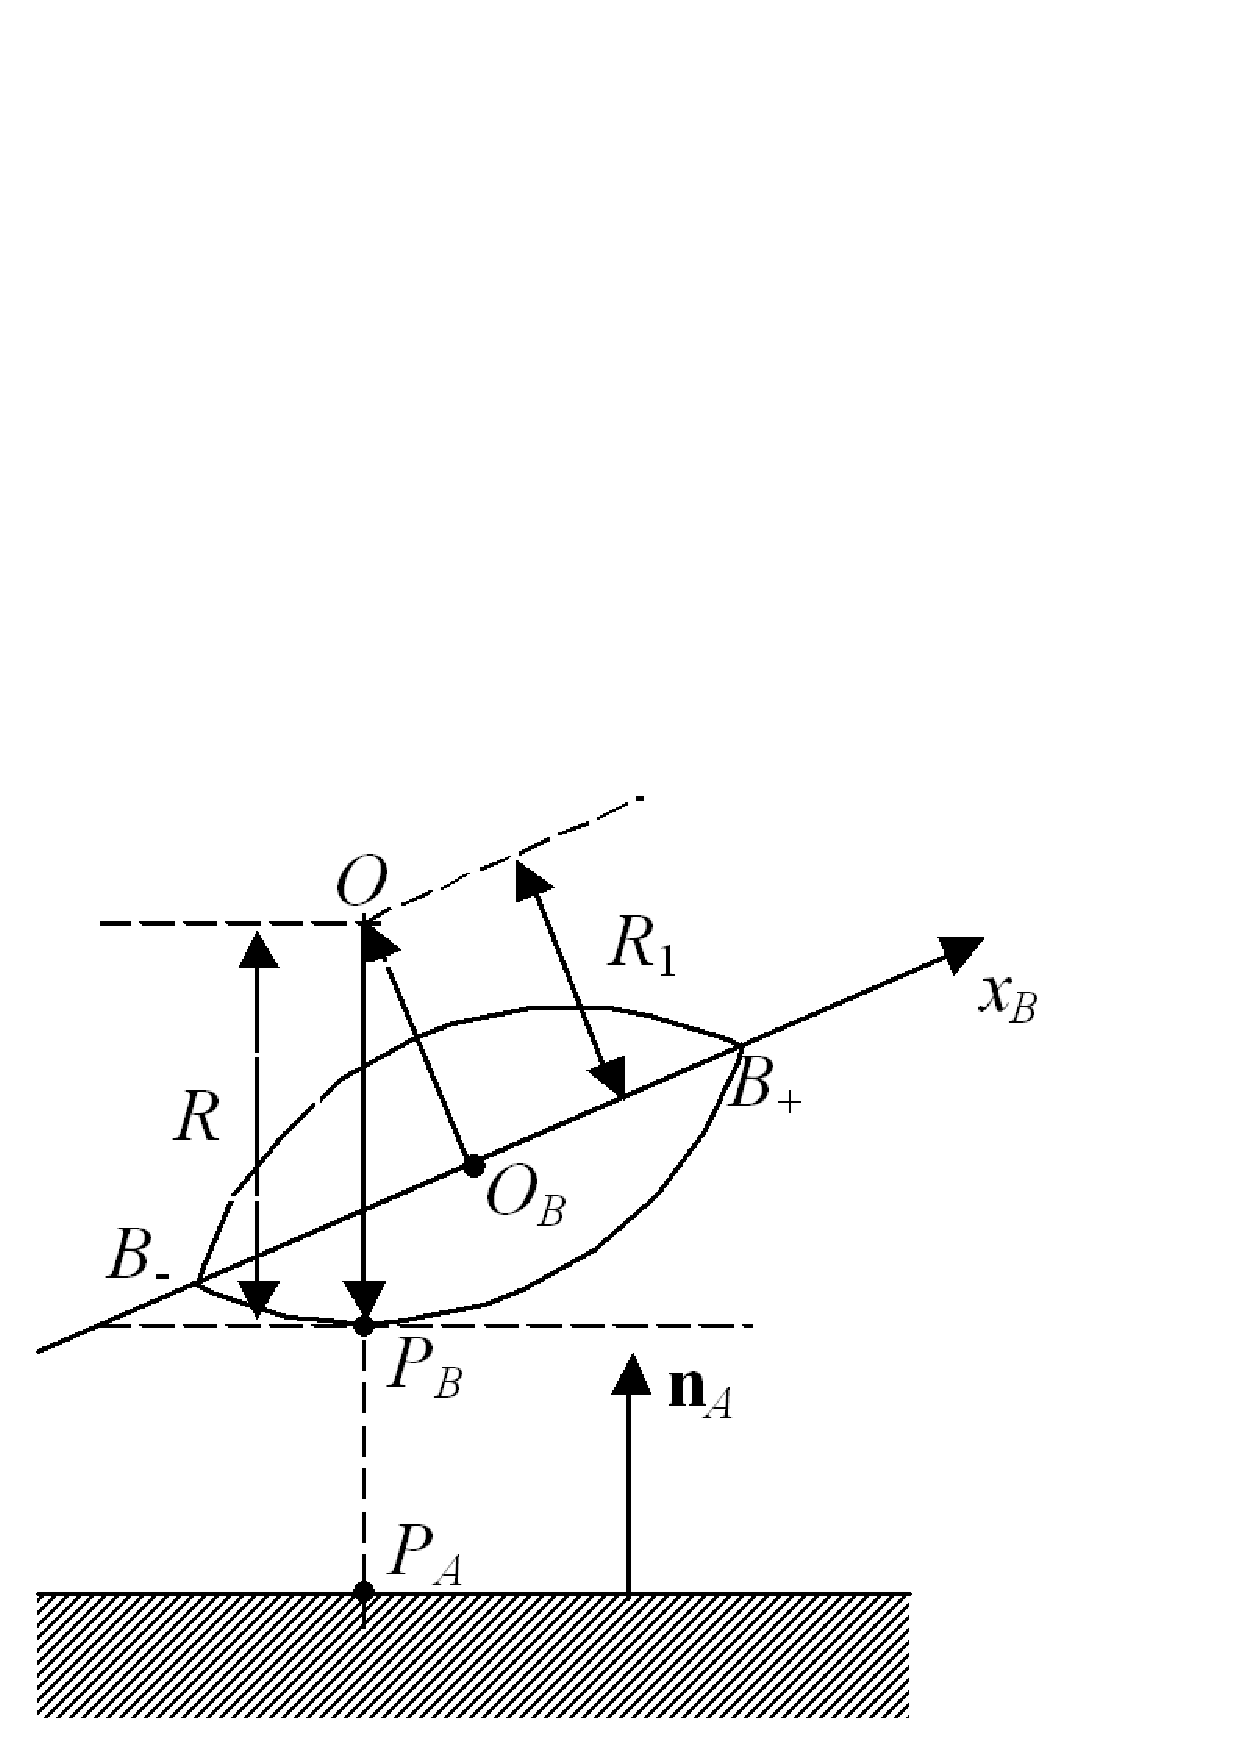
\includegraphics[bb= 0cm 0cm 20cm 17cm,scale=0.30]{RollerSection.png}}
% \caption{Contact tracking scheme.}
% \label{ContactScheme}
% \end{figure}

% Во время счета компоненты всех векторов задаются относительно неподвижной системы отсчета, а положения и ориентации всех тел системы в момент времени $t\in [t_0,t_1]$ считаются известными.

% Таким образом, для системы $K{\bf i}_2{\bf j}_2{\bf k}_2$, имеем:
% $$
% {\bf i}_2=T_B\cdot (1,0,0)^T,\quad\vecrho =
% \left( {\bf r}_{O_A}-{\bf r}_{O_B}\right) /
% \left| {\bf r}_{O_A}-{\bf r}_{O_B}\right| ,
% $$
% где $T_B$ -- матрица ориентации ролика, а единичный вектор $\vecrho$ направлен вдоль луча, выпущенного из центра колеса $O_A$ в сторону центра ролика $O_B$.

Как и в случае $\psi = 0$, определим направление ``на центр колеса'' от центра ролика, т.е. вектор
$$
    \vecrho = \ddfrac
        { {\bf r}_{P}-{\bf r}_{K} }
        {\left| {\bf r}_{P}-{\bf r}_{K} \right|}.
$$

Вектор ${\bf i}_1$ расположим на пересечении плоскости колеса и горизонтальной плоскости. Пусть вектор ${\bf k}_1 = {\bf k}$ ортогонален плоскости колеса и совпадает с одним из векторов базиса, связанного с колесом, и всегда горизонтален. 
% Тогда имеем ${\bf j}_1(t)=(0,1,0)^T$ и ${\bf i}_1(t)={\bf j}_1(t)\times {\bf k}_1(t)$.
$\vec{j}_1$ положим совпадающим с $\vec{\gamma}$. Тогда $\vec{i}_1$ может быть определен как ${\bf i}_1 = {\bf j}_1 \times {\bf k}_1$.

Теперь рассмотрим соотношения, позволяющие вычислить компоненты базисных векторов системы отсчета $K{\bf i}_2{\bf j}_2{\bf k}_2$.

Отметим, что вектор ${\bf i}_2$, направленный вдоль оси ролика, по определению не может принять вертикальное положение, если ролик находится в контакте с опорной плоскостью. Более того, в случае \textit{mecanum} ролик повернут на постоянный угол $\psi > 0$ относительно оси $PK$, и потому во все время движения верно соотношение ${\bf i}_2 \ne \vec{\gamma}$. Таким образом, вектор ${\bf c} = {\bf i}_2 \times \vec{\gamma}$ также отличен от нуля. Положим ${\bf k}_2 = \ddfrac{\vecrho}{|\vecrho|}$. Теперь можно определить ${\bf j}_2$ как ${\bf j}_2 = {\bf k}_2 \times {\bf i}_2$.

Для определения компонент вектора $\vecrho$ воспользуемся кинематическими соотношениями, условиями ортогональности векторов, следующими из определений введенных систем отсчета:
$$
    \vecrho \cdot {\bf i}_2 = 0, \quad \vecrho \cdot {\bf k}_1 = 0,
$$
а точнее, их дифференциальными вариантами:
$$
    \dfrac{d}{dt}\vecrho \cdot {\bf i}_2 + \vecrho \cdot \dfrac{d}{dt}{\bf i}_2 = 0,\quad
    \dfrac{d}{dt} \vecrho \cdot {\bf k}_1 + \vecrho \cdot \dfrac{d}{dt}{\bf k}_1 = 0.
$$

Величина $c_{\beta} = \cos\beta = {\bf i}_2 \cdot \vec{\gamma}$ косинуса угла $\beta$ наклона оси ролика к вертикали $\vec{\gamma}$ также играет важную роль в алгоритме отслеживания контакта. Если текущее значение $c_{\beta }$ меньше некоторого уровня $c_{\beta\max}$, и если одновременно расстояние от центра ролика $K$ до опорной плоскости меньше радиуса колеса $l$, то ролик находится в контакте с опорной плоскостью. В противном случае контакт отсутствует.

Итак, ролик находится в контакте, если только если $\vec{s} \cdot \vec{e}_z < \cos\ddfrac{\pi}{n} $ и $ z_C < l $. В противном случае со стороны опорной плоскости к ролику не приложены силы. В случае контакта, сперва найдем координаты точки ролика, находящейся в данный момент на опорной плоскости:

$$ \vec{r}_C = \vec{r}_K + r\vec{s} - l\vec{e}_z + \lambda\vec{k}_1 $$

Чтобы получить число $\lambda$, умножим последнее уравнение скалярно на ${\bf k}_2$. Отсюда

$$ \lambda = \ddfrac{\left(r\vec{s} - l\vec{e}_z\right)\cdot\vec{k}_2}{ \vec{k}_1\cdot\vec{k}_2} $$
$$ \vec{v}_C = \vec{v}_K + [ \vec{\omega}_{\text{рол}}, \overrightarrow{KC} ],$$

поскольку ${\bf r}_{C}-{\bf r}_{K}$ лежит в вертикальном сечении осесимметричной поверхности ролика, и вектор ${\bf k}_2$ по построению ортогонален этому сечению. В результате радиус-вектор ${\bf r}_{C}$ точки контакта определяется однозначно.

% На рис.~\ref{ContactScheme} также легко видеть, что координаты точки $C$ контакта ролика и плоскости даются выражением
% $$
% {\bf r}_{P_B}={\bf r}_{O_B}+R_1\vecrho -R{\bf j}_1+\mu {\bf k}_1,
% $$
% где число $\mu$ требуется вычислить (см. рис.~\ref{fig:mecanum}). Здесь величина $R_1$ равна расстоянию между точками $O_A$ и $O_B$.
Для решения задачи отслеживания контакта снова требуется указать два выражения: формулу для нахождения координат точки контакта и условие наличия контакта как такового. В случае \textit{mecanum}, в отличие от случая омни-колеса, точка контакта $C$, вообще говоря, не лежит в плоскости, содержащей диск колеса. Способ нахождения радиуса-вектора $\vec{r}_C$ точки контакта, предлагаемый в настоящем разделе, основан на вычислении расстояния $\lambda$ от этой плоскости до $C$. Условие наличия контакта аналогично полученному в предыдущем разделе, но для его проверки требуется учесть отличия в геометрии ролика: $\psi \ne 0$.

\textbf{Неявный алгоритм отслеживания контакта}

Как и в случае $\psi = 0$, определим направление ``на центр колеса'' от центра ролика, т.е. вектор
$$
    \vecrho = \ddfrac
        { {\bf r}_{P}-{\bf r}_{K} }
        {\left| {\bf r}_{P}-{\bf r}_{K} \right|}.
$$
Таким образом, ролик находится в контакте, если только если
$$
     \vec{s} \cdot \vec{e}_z < \cos\ddfrac{\pi}{n} \enspace \text{и} \enspace z_C < l.
$$
Также определим вектор $\vec{k}$, направленный вдоль оси колеса (т.е. перпендикулярно плоскости колеса). Тогда радиус-вектор $\vec{r}_C$ точки контакта $C$ можно выразить следующим образом через введенные векторы и радиус-вектор $\vec{r}_K$ центра ролика $K$:
\begin{equation}\label{eq:cont_impl}
    \vec{r}_C = \vec{r}_K + r\vec{s} - l\vec{e}_z + \lambda\vec{k}.
\end{equation}
В этом выражении компоненты векторов $\vec{s}$ и $\vec{k}$, а также расстояние от плоскости колеса до точки контакта $\lambda$ не известны, их требуется вычислять. Для этого введем три вспомогательные системы отсчета и, пользуясь ими, получим необходимые выражения.

Введем систему отсчета $P{\bf i}{\bf j}{\bf k}$, жестко связанную с диском колеса (см. фиг.~\ref{fig:mecanum}), с началом в его центре $P$. Пусть вектор ${\bf k}$ направлен вдоль оси колеса, ${\bf i}$ и ${\bf j}$ лежат в его плоскости. Дополнительно введем также системы отсчета $P{\bf i}_1{\bf j}_1{\bf k}_1$ и $K{\bf i}_2{\bf j}_2{\bf k}_2$, где $K$ -- центр ролика.

Вектор ${\bf i}_1$ направим вдоль линии пересечения плоскости колеса и горизонтальной плоскости. Пусть вектор ${\bf k}_1 = {\bf k}$ совпадает c вектором $\vec{k}$ базиса, связанного с колесом, ортогонален плоскости колеса и всегда горизонтален. 
$\vec{j}_1$ положим совпадающим с вектором восходящей вертикали $\vec{\gamma}$. Тогда $\vec{i}_1$ определим как ${\bf i}_1 = {\bf j}_1 \times {\bf k}_1$.

Вектор ${\bf i}_2$ направим вдоль оси собственного вращения ролика, см. фиг.~\ref{fig:mecanum}. Этот вектор по определению не может принять вертикальное положение при $\psi = 0$, если ролик находится в контакте с опорной плоскостью, а, в случае \textit{mecanum} ролик повернут на постоянный угол $\psi > 0$ относительно оси $PK$, и потому соотношение ${\bf i}_2 \ne \vec{\gamma}$ верно во все время движения. Это обстоятельство позволяет определить вектор ${\bf c} = {\bf i}_2 \times \vec{\gamma}$, всегда отличный от нуля. Положим ${\bf k}_2 = \ddfrac{\vec{c}}{|\vec{c}|}$. Вектор ${\bf j}_2$ положим ортогональным ${\bf i}_2$ и лежащим в вертикальной плоскости как ${\bf j}_2 = {\bf k}_2 \times {\bf i}_2$.

Для определения компонент вектора $\vecrho$ теперь воспользуемся условиями ортогональности векторов, следующими из определений введенных систем отсчета:
$$
    \vecrho \cdot {\bf i}_2 = 0, \quad \vecrho \cdot {\bf k}_1 = 0,
$$
а точнее, их дифференциальными вариантами:
$$
    \dfrac{d}{dt} \vecrho \cdot {\bf i}_2 + \vecrho \cdot \dfrac{d}{dt} {\bf i}_2 = 0, \quad
    \dfrac{d}{dt} \vecrho \cdot {\bf k}_1 + \vecrho \cdot \dfrac{d}{dt} {\bf k}_1 = 0.
$$

Чтобы получить число $\lambda$, умножим уравнение\upr{eq:cont_impl} скалярно на ${\bf k}_2$. Поскольку ${\bf r}_C - {\bf r}_K$ лежит в вертикальном сечении осесимметричной поверхности ролика, и вектор ${\bf k}_2$ по построению ортогонален этому сечению, расстояние $\lambda$ от плоскости колеса до точки контакта $C$ определяется однозначно как
$$
    \lambda = \ddfrac
        { \left( r\vec{s} - l\vec{e}_z \right) \cdot \vec{k}_2 }
        { \vec{k}_1 \cdot \vec{k}_2 },
$$
а вместе с ним, и весь радиус-вектор $\vec{r}_C$. Аналогично предыдущему разделу, налагается связь вида \upr{eq:cont_vn,eq:cont_Dvn}.


\textbf{Явный алгоритм отслеживания контакта}

Для полноты изложения приведем еще один способ вычисления компонент радиуса-вектора ${\bf r}_{C}$ точки контакта $C$ или, точнее, точки ролика, ближайшей к опорной плоскости, предложенный С.Я.Сте\-па\-но\-вым \cite{KosenkoGerasimov2015}. Способ заключается в применении следующего набора равенств (см. рис.~\ref{fig:mecanum}):
% Лучше всего этот способ иллюстрирует геометрическая схема на рис.~\ref{fig:figure3}.
% STEPANOV
% Во-первых, имеем
% $$
% {\bf r}_{P_B}={\bf r}_{O_B}+\overrightarrow{CD}+\overrightarrow{DG},\quad
% \overrightarrow{CD}=-m{\bf i}_2,\quad\overrightarrow{DG}=-h{\bf j}_1,
% $$
$$
{\bf r}_{C}={\bf r}_{K}+\overrightarrow{KD}+\overrightarrow{DC},\quad
\overrightarrow{KD}=-a{\bf i}_2,\quad\overrightarrow{DC}=-h{\bf j}_1,
$$
% STEPANOV
% где $m=R_1\sin q / \cos q/\cos\psi $, $h=R-R_1/\cos q$. 
% Здесь $q$ -- текущее значение угла отклонения вектора ${\bf r}_{O_A}-{\bf r}_{O_B}$ от 
где $a = r\ddfrac{\sin\chi}{\cos\chi\cos\psi}$, $h = l - \ddfrac{r}{\cos\chi}$. Здесь $\chi$ -- текущее значение угла отклонения вектора $\vec{c}$ из предыдущего раздела от 
вертикали. Таким образом,
$$
    \cos\chi = \vecrho \cdot \vec{\gamma}, \quad \sin\chi = 
    \left( \vec{\gamma} \times \vecrho \right) \cdot {\bf k}_1.
$$
% STEPANOV
% $$
% \cos q=\vecrho\cdot{\bf n}_A,\quad\sin q=
% \left({\bf n}_A\times\vecrho\right)\cdot {\bf k}_1.
% $$
% \begin{figure*}[H]
% \centerline{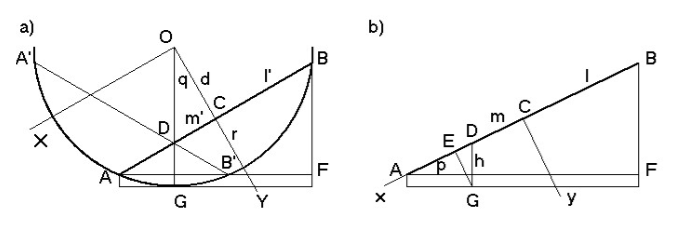
\includegraphics[scale=0.7]{content/parts/3_friction/mo2015/stepanov.png}}
% \caption{Явная схема отслеживания контакта}
% \label{fig:figure3}
% \end{figure*}
% STEPANOV
% Поясним рис.~\ref{fig:figure3} более детально.
% В части (а) приведена проекция колеса на его плоскость и соответственно, проекция ролика, находящегося в общем положении так, что его ось находится под углом к плоскости проекции.
% Далее, $G$ -- точка контакта между роликом и опорной горизонтальной плоскостью в настоящий момент, $m'$ -- отрезок $DC$ проекции оси ролика на плоскость колеса. Легко видеть, что длина этой проекции равна $m'=m\cos\psi$, поскольку ось ролика $AB$ повернута вокруг прямой $OC$ на угол $\psi$, см. вертикальное сечение, содержащее ось ролика в части (b).
% Таким образом, чтобу получить точку контакта $P_B$ ($G$ на рис.), нужно пройти два отрезка прямых от центра ролика $O_B$ ($C$ на рис.): (a)~отрезок $CD$ оси ролика длины $m$; 
% (b)~отрезок $DG$ вертикали длины $h$.
% Как было отмечено выше, все величины требуется явно выразить через известные координаты.
Кривая, образующая поверхность ролика, пересекает его ось в окрестности острия и продолжается далее (параметризация образующей кривой, поверхности ролика и сечения этой поверхности плоскостью, содержащей ось ролика, приведены в \cite{Gfrerrer2008}), в связи с чем
% Чтобы исключить <<перекрытие>> роликов, т.е. ситуацию, при которой два ролика могут находиться в контакте одновременно, более чем при одном (граничном) значении угла поворота колеса,
необходимо ограничить длины роликов величиной
$$
L=2l\ddfrac{\sin\ddfrac{\pi}{n}}{\cos\psi},
$$
где $\ddfrac{\pi}{n}$ -- половина угла раствора дуги окружности, ограничивающей проекцию ролика на плоскость колеса. При такой конструкции колеса переход колеса с одного ролика на другой происходит мгновенно.
% и при этом их концы оказываются усечены.
% Подробно форма кривой, образующей поверхность роликов, описана в \cite{Gfrerrer2008}.
Отметим, что при этом след колеса на плоскости имеет разрыв, поскольку точка контакта мгновенно переходит на противоположный <<борт>> колеса. Это обстоятельство, впрочем, не препятствует эффективному численному решению.

% Описанные алгоритмы отслеживания контакта дают практически одинаковые результаты, относительные различия между которыми имеют порядок $10^{-8}$. Предсказуемо, явный алгоритм быстрее приблизительно в $1.5$ раза.
